% Options for packages loaded elsewhere
\PassOptionsToPackage{unicode}{hyperref}
\PassOptionsToPackage{hyphens}{url}
%
\documentclass[
]{article}
\usepackage{lmodern}
\usepackage{amssymb,amsmath}
\usepackage{ifxetex,ifluatex}
\ifnum 0\ifxetex 1\fi\ifluatex 1\fi=0 % if pdftex
  \usepackage[T1]{fontenc}
  \usepackage[utf8]{inputenc}
  \usepackage{textcomp} % provide euro and other symbols
\else % if luatex or xetex
  \usepackage{unicode-math}
  \defaultfontfeatures{Scale=MatchLowercase}
  \defaultfontfeatures[\rmfamily]{Ligatures=TeX,Scale=1}
\fi
% Use upquote if available, for straight quotes in verbatim environments
\IfFileExists{upquote.sty}{\usepackage{upquote}}{}
\IfFileExists{microtype.sty}{% use microtype if available
  \usepackage[]{microtype}
  \UseMicrotypeSet[protrusion]{basicmath} % disable protrusion for tt fonts
}{}
\makeatletter
\@ifundefined{KOMAClassName}{% if non-KOMA class
  \IfFileExists{parskip.sty}{%
    \usepackage{parskip}
  }{% else
    \setlength{\parindent}{0pt}
    \setlength{\parskip}{6pt plus 2pt minus 1pt}}
}{% if KOMA class
  \KOMAoptions{parskip=half}}
\makeatother
\usepackage{xcolor}
\IfFileExists{xurl.sty}{\usepackage{xurl}}{} % add URL line breaks if available
\IfFileExists{bookmark.sty}{\usepackage{bookmark}}{\usepackage{hyperref}}
\hypersetup{
  hidelinks,
  pdfcreator={LaTeX via pandoc}}
\urlstyle{same} % disable monospaced font for URLs
\usepackage[margin=1in]{geometry}
\usepackage{graphicx,grffile}
\makeatletter
\def\maxwidth{\ifdim\Gin@nat@width>\linewidth\linewidth\else\Gin@nat@width\fi}
\def\maxheight{\ifdim\Gin@nat@height>\textheight\textheight\else\Gin@nat@height\fi}
\makeatother
% Scale images if necessary, so that they will not overflow the page
% margins by default, and it is still possible to overwrite the defaults
% using explicit options in \includegraphics[width, height, ...]{}
\setkeys{Gin}{width=\maxwidth,height=\maxheight,keepaspectratio}
% Set default figure placement to htbp
\makeatletter
\def\fps@figure{htbp}
\makeatother
\setlength{\emergencystretch}{3em} % prevent overfull lines
\providecommand{\tightlist}{%
  \setlength{\itemsep}{0pt}\setlength{\parskip}{0pt}}
\setcounter{secnumdepth}{-\maxdimen} % remove section numbering
\usepackage[french, USenglish]{babel}
\usepackage{fancyhdr}
\pagestyle{fancy}
\renewcommand{\sectionmark}[1]{\markright{#1}}
\fancyhf{}
\lhead{{}}
\rhead{{\today}}
\cfoot{{\thepage}}
\usepackage[T1]{fontenc}
\usepackage{bm}
\usepackage{mathpazo}
\usepackage{tabularx}
\usepackage{titlesec}
\usepackage{graphicx, xcolor}
\usepackage{wrapfig}
\usepackage{amssymb}
\usepackage{amsmath}
\usepackage{lscape}
\usepackage{esint}
\usepackage{paralist}
\usepackage{outlines}
\newcommand{\I}{\textrm{I}}
\newcommand{\N}{\mathcal{N}}
\newcommand{\D}{\textrm{D}}
\newcommand{\E}{\mathbb{E}}
\setlength{\parskip}{1em} %0.5\baselineskip
\setlength{\parindent}{0pt}
\linespread{1.15}
\titleformat*{\section}{\Large\scshape\bfseries}
\titleformat*{\subsection}{\large\scshape\bfseries}
\titleformat*{\subsubsection}{\bfseries}
\titleformat*{\paragraph}{\bfseries}
\titleformat*{\subparagraph}{\bfseries}
\renewcommand{\thesection}{\Roman{section}.} % 1.A. as subsections
\renewcommand{\thesubsection}{\Alph{subsection}.} % 1.A. as subsections
\titlespacing{\section}{0pt}{2pt}{3pt}
\titlespacing{\subsection}{0pt}{2pt}{2pt}
\titlespacing{\subsubsection}{0pt}{0pt}{0pt}
\titlespacing{\paragraph}{0pt}{1pt}{5pt}
\titlespacing{\subparagraph}{10pt}{1pt}{5pt}
\usepackage{hyperref}
\hypersetup{ colorlinks=true, citecolor = blue, linkcolor=blue, urlcolor=blue}
\usepackage[font={footnotesize}]{subcaption}
\usepackage[font={footnotesize}]{caption}
\usepackage{caption, setspace}
\captionsetup{font={stretch=1}}
\captionsetup[figure]{font=footnotesize,labelfont=footnotesize}
\usepackage{tabto}
\def\quoteattr#1#2{\setbox0=\hbox{#2}#1\tabto{\dimexpr\linewidth-\wd0}\box0}
\makeatletter
\newcommand{\pushright}[1]{\ifmeasuring@#1\hfill$\displaystyle#1$\fi\ignorespaces}
\makeatother
\newcommand{\FixMe}[1]{\textcolor{orange}{ [#1]}}
\newcommand{\Comment}[1]{\textcolor{purple}{\textit{[#1]}}}
\newcommand{\Quickwin}{{\color{blue}{$\bigstar$}} }
\renewcommand{\thetable}{S\arabic{table}}
\usepackage{letltxmacro}
\LetLtxMacro\Oldfootnote\footnote
\newcommand{\EnableFootNotes}{\LetLtxMacro\footnote\Oldfootnote}
\newcommand{\DisableFootNotes}{\renewcommand{\footnote}[2][]{\relax}}
\makeatother
\graphicspath{{../Output/"}}
\usepackage{booktabs}
\usepackage{longtable}
\usepackage{array}
\usepackage{multirow}
\usepackage{wrapfig}
\usepackage{float}
\usepackage{colortbl}
\usepackage{pdflscape}
\usepackage{tabu}
\usepackage{threeparttable}
\usepackage{threeparttablex}
\usepackage[normalem]{ulem}
\usepackage{makecell}

\author{}
\date{\vspace{-2.5em}}

\begin{document}

\begin{center} 
    \textbf{\scshape \LARGE Extended Supplemental Information}\\  \vspace{2mm}
    {\large COVID-19 and All-Cause Mortality in the US and 18 Comparison Countries}\\ \vspace{2mm} 
    {\large Alyssa Bilinski $\cdot$ Ezekiel Emanuel\footnote{Contact: zemanuel@upenn.edu},\footnote{Data and code are available on GitHub (\href{https://github.com/abilinski/MortalityCOVID19}{link}).}} \\
\end{center}

\vspace{-0.50em}

\bigskip

\hypertarget{calculations-in-tables-1-and-2}{%
\subsection{Calculations in Tables 1 and
2}\label{calculations-in-tables-1-and-2}}

\hypertarget{difference-in-deaths}{%
\subsubsection{Difference in deaths}\label{difference-in-deaths}}

Let \(r_i\) be the death rate of interest (reported COVID-19 deaths or
excess all cause mortality) per 100,000 in country \(i\), and \(d\) be
US deaths over the period of study. Let \(p\) be the US 2019 population,
\(p=329,064,917\) according to the European Centre for Disease
Prevention and Control. We estimate difference in deaths: \begin{align}
d - \left(r_i/100,000\right)*p
\end{align}

\hypertarget{difference-in-deaths-if-comparable-after-some-time-point}{%
\subsubsection{Difference in deaths if comparable after some time
point}\label{difference-in-deaths-if-comparable-after-some-time-point}}

Letting \(r_{iT}\) be the death rate per 100,000 in country \(i\)
between time \(T\) and the end of the period of study and \(d_T\) be US
deaths by time \(T\), we estimate potential difference in deaths since
time \(T\): \begin{align}
d - \left(d_T + \left(r_{iT}/100,000\right)*p\right)
\end{align}

\hypertarget{difference-in-deaths-if-matching-after-some-criteria-is-met-i.e.-adjustment-for-pandemic-timing}{%
\subsubsection{Difference in deaths if matching after some criteria is
met (i.e., adjustment for pandemic
timing)}\label{difference-in-deaths-if-matching-after-some-criteria-is-met-i.e.-adjustment-for-pandemic-timing}}

Let time \(T_i\) be the time that country \(i\) meets some criteria
(i.e., 60 days after \(\geq\) 1 case per 100,000 population). Let \(T\)
be the time that the US meets the criteria. Letting \(r_{iT_i}\) be the
death rate per 100,000 in a comparison country between time \(T_i\) and
the end of the reporting period and \(d_{T}\) be US deaths until time
\(T\), we estimate potential difference in deaths since time \(T\):
\begin{align}
d - \left(d_{T} + \left(r_{iT_i}/100,000\right)*p\right)
\end{align}

\hypertarget{technical-notes}{%
\subsection{Technical notes}\label{technical-notes}}

\hypertarget{analytic-approach}{%
\subsubsection{Analytic approach}\label{analytic-approach}}

\begin{enumerate}
\def\labelenumi{\arabic{enumi}.}
\tightlist
\item
  There has been debate in the epidemiological community regarding
  whether to adjust deaths per capita early in the pandemic. Given a
  fixed number introductions, we do not expect that early in a pandemic,
  a virus would spread faster in a larger population than in a smaller
  one. Nevertheless, we defer to per capita measures due to the
  geographic and demographic diversity of the United States that renders
  it likely more similar to a combination of small countries than a
  single countries, and as viral introductions may be proportional to
  population. In addition, this measure may better capture the pandemic
  measure along other dimensions (e.g.~perceived social impact).
\item
  Due to large sample sizes, traditional statistical inference around
  differences in mortality rates often has narrow confidence intervals
  and meets traditional standards for ``statistical significance'' (see
  e.g.,
  \href{https://jamanetwork.com/journals/jamainternalmedicine/fullarticle/2767980}{Weinberger et. al}).
  As our other outcome measures (e.g.~excess deaths) are invertible
  monotone transformation of mortality rates, statistical conclusions
  about the former apply to the latter. However, other sources of
  uncertainty affect our results more than statistical randomness, which
  we aim to capture in sensitivity analyses.
\item
  We consider a number of sensitivity analyses in the tables below. Our
  main analysis focuses on \emph{calendar time}, assuming that the US
  death rate became comparable to another country's death rate after a
  particular point in time. We consider both May and June for this
  change, allowing approximately 2-3 months for responses after cases
  and deaths emerged in the United States. We use calendar time as our
  main specification because 1) the pandemic affected most countries at
  similar times (Table \ref{tbl.S1}), and 2) to the extent that there
  were differences, countries are able to react to the experiences of
  other peer countries (e.g.~by responding earlier even if the pandemic
  affected them later). However, we may want to
  \emph{adjust for pandemic timing} if, for example, countries were
  unable to gain political will to implement measures before evidence of
  a more local pandemic and/or if the pandemic was particularly
  difficult to control until cases reached a specific threshold. We
  therefore consider 2 sensitivity analyses in (Table \ref{tbl.S1},
  \ref{tbl.S2}, \ref{tbl.S3}): 1) assuming the US had a comparable
  mortality rate to a country 60 days after reaching 1 case per million
  (Scenario D) and 2) assuming the US had a comparable mortality rate to
  a country 60 days after reaching 5 deaths (Scenario E). The former is
  generally lower than May estimates while the latter is higher.
\item
  For excess all-cause mortality, we use 2015-2019 as comparison years
  by default, based on the CDC's excess death analysis. In sensitivity
  analysis, we present results using 2018-2019 (Table \ref{tbl.S3}),
  which has a slightly lower estimate of excess all-cause mortality but
  similar overall patterns.
\end{enumerate}

\bigskip

\hypertarget{country-level-data}{%
\subsubsection{Country-level data}\label{country-level-data}}

\begin{enumerate}
\def\labelenumi{\arabic{enumi}.}
\tightlist
\item
  Spain adjusted its cumulative COVID-19 death toll downward (and then
  partially upward) during May and June 2020. We smoothed this to be
  monotonic over this time period by setting cumulative deaths between
  May 23, 2020 and June 18, 2020 to be equal to the reported death toll
  on June 19, 2020 (Figure \ref{supp.fig.spain}).
\item
  For recent periods in which some deaths may not yet have been
  reported, the United States CDC provides estimates of both unweighted
  deaths and deaths weighted to attempt to adjust for underreporting. To
  be conservative in our estimate of excess deaths, we use the latter
  (Figure \ref{supp.fig.weighting}). In our excess all-cause mortality
  analyses, we use through week 30 (July 25, 2020). While difficult to
  pinpoint a precise cut-off at which data were sufficiently complete
  for inclusion, both CDC reported deaths and COVID-19 attributed deaths
  (see ``USA\_2.csv'') declined through August, suggesting decreases in
  reporting by at least week 32-33, and this was also the last time
  point at which data were available for Canada, allowing us to include
  in our excess all-cause mortality analysis.
\item
  Several countries reported lower than average all-cause mortality in
  2020 prior to the pandemic (Figure \ref{supp.weekly.deaths}). For this
  reason, we start measurement of all-cause mortality after the pandemic
  began in a country (\(\geq\) 5 cases per million recorded).
\item
  We lacked sufficient data from Australia, Japan, and South Korea to do
  direct comparisons in our excess deaths analysis (Table 2 of main
  paper), but analyses of available data suggest that these low
  mortality countries did not experience meaningful excess mortality
  during 2020
  (e.g.~\href{https://www.abc.net.au/news/2020-06-23/coronavirus-australia-excess-deaths-data-analysis/12321162}{Australia},
  \href{https://www.bloomberg.com/news/articles/2020-07-29/japan-dodged-surge-in-total-fatalities-during-peak-virus-month}{Japan},
  \href{https://www.nytimes.com/interactive/2020/04/21/world/coronavirus-missing-deaths.html}{South Korea})
\item
  France provided a
  \href{https://www.insee.fr/fr/statistiques/4487988?sommaire=4487854}{file}
  of estimated deaths beginning in February for the years 2018-2020.
  Following \emph{The Economist}
  \href{https://github.com/TheEconomist/covid-19-excess-deaths-tracker}{GitHub},
  we used France's
  \href{https://www.insee.fr/fr/information/4190491}{death registers} to
  fill in 2015-2017. When we compared the death registers in 2018 to the
  first file, we found that the latter had lower deaths by week, and
  therefore to be conservative in estimates of excess deaths and
  following the approach of \emph{The Economist}, we only included
  deaths with a valid department code in ``location of death.''
\end{enumerate}

\bigskip

\hypertarget{other}{%
\subsubsection{Other}\label{other}}

\begin{enumerate}
\def\labelenumi{\arabic{enumi}.}
\tightlist
\item
  Research letters are limited to 6 references, and cited papers must be
  peer-reviewed. However, there were a number of other sources
  consulted, including on the potential impact of early interventions
  prior to a US surge
  (\href{https://www.medrxiv.org/content/10.1101/2020.05.15.20103655v2}{Pei et. al.},
  \href{https://www.nytimes.com/2020/04/14/opinion/covid-social-distancing.html?searchResultPosition=2}{NYT},
  \href{https://www.statnews.com/2020/06/19/faster-response-prevented-most-us-covid-19-deaths/}{StatNews});
  on excess mortality (\emph{News:}
  \href{https://www.economist.com/graphic-detail/2020/07/15/tracking-covid-19-excess-deaths-across-countries}{Economist},
  \href{https://www.nytimes.com/interactive/2020/04/21/world/coronavirus-missing-deaths.html}{NYT},
  \href{https://ourworldindata.org/excess-mortality-covid}{Our World in Data},
  \href{https://www.nature.com/articles/d41586-020-02497-w}{Nature News};
  \emph{Academic:}
  \href{https://www.inet.ox.ac.uk/files/15.44-final-25-Aug-20-Aron-Muellbauer-Transatlantic-excess-mortality-comparison-r.pdf}{Aron and Muellbauer},
  \href{https://jamanetwork.com/journals/jamainternalmedicine/fullarticle/2767980}{Weinberger et. al},
  \href{https://jamanetwork.com/journals/jama/fullarticle/2768086}{Woolf et. al},
  \href{https://www.medrxiv.org/content/10.1101/2020.08.31.20184036v3}{Stokes et. al.}).
  Similar issues were also debated recently in NYT
  (\href{https://www.nytimes.com/2020/09/01/briefing/coronavirus-kenosha-massachusetts-your-tuesday-briefing.html}{link},
  \href{https://www.nytimes.com/2020/09/05/opinion/sunday/covid-19-trump.html}{link})
  and in
  \href{https://www.vox.com/future-perfect/2020/9/9/21428769/covid-19-coronavirus-deaths-statistics-us-canada-europe}{Vox}.
\end{enumerate}

\bigskip

\clearpage

\begin{figure}
\centering
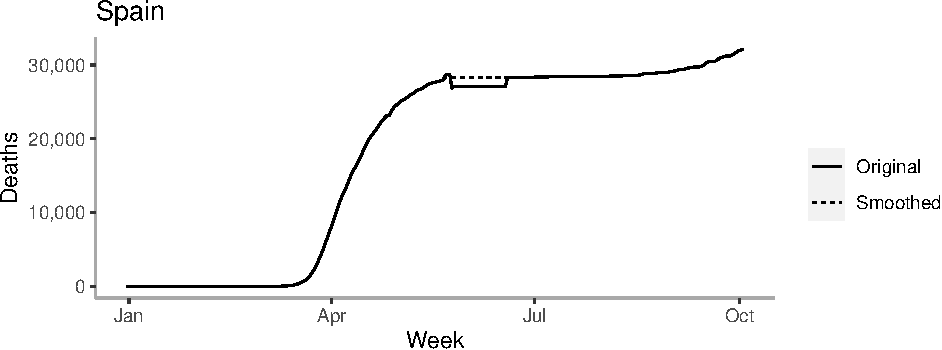
\includegraphics{extended_supplement_FINAL_files/figure-latex/notes2-1.pdf}
\caption{\label{supp.fig.spain} Spanish COVID-19 deaths, with and
without smoothing.}
\end{figure}

\begin{figure}
\centering
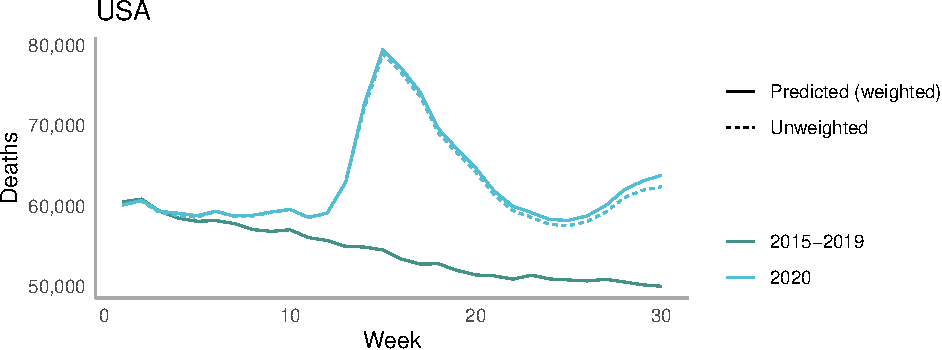
\includegraphics{extended_supplement_FINAL_files/figure-latex/notes-1.pdf}
\caption{\label{supp.fig.weighting} Deaths by week with and without
weighting for underreporting. The line marked 2015-2019 represented the
average over those years.}
\end{figure}

\clearpage

\begin{figure}
\centering
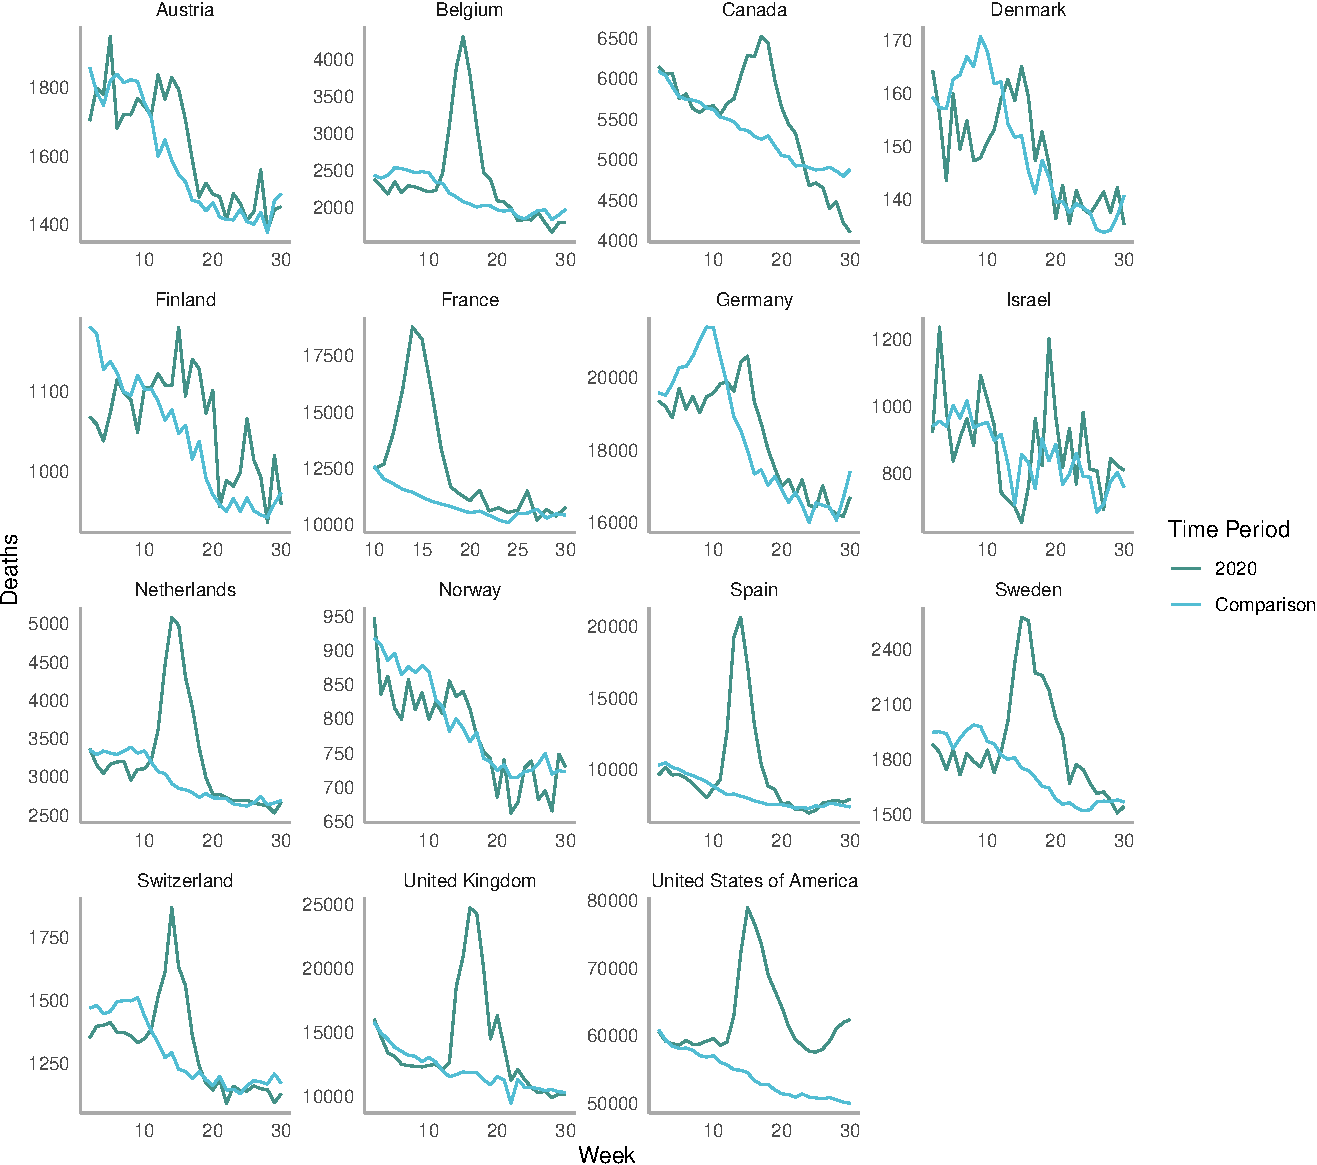
\includegraphics{extended_supplement_FINAL_files/figure-latex/unnamed-chunk-1-1.pdf}
\caption{\label{supp.weekly.deaths} All-cause mortality by country by
week and year. The comparison period is the average of 2015-2019, except
in Germany, we used only years 2016-19 due data accessibility. Early
2020 mortality is lower than average in e.g.~Denmark, Germany, and
Switzerland.}
\end{figure}

\clearpage

\hypertarget{mortality-time-series}{%
\subsection{Mortality Time Series}\label{mortality-time-series}}

\begin{figure}
\centering
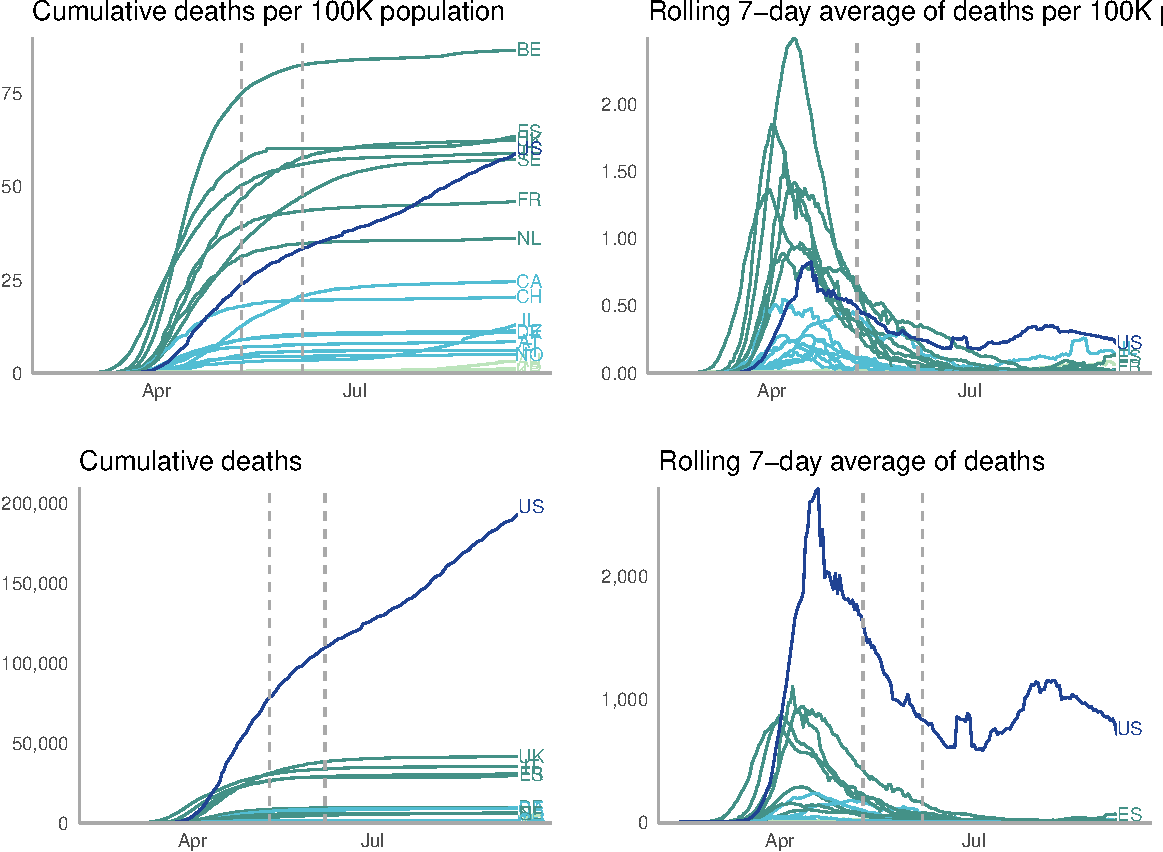
\includegraphics{extended_supplement_FINAL_files/figure-latex/percapitaplot-1.pdf}
\caption{Estimates of per capita and total COVID-19 mortality from
February-September 2020.}
\end{figure}

\pagebreak

\begin{landscape}
\begin{table}[H]

\caption{\label{tab:unnamed-chunk-2}\label{tbl.S1}Data on coronavirus disease 2019 (COVID-19) deaths are from February 13, 2020, through September 19, 2020 (n = 198 589 US deaths).  Death rates per 100K Scenarios: (A) full sample; (B) since May 10, 2020; (C) since June 7, 2020; (D) since 60 days after surpassing 1 case per million; (E) since 60 days after surpassing 5 COVID-19 deaths.  The last 5 columns assume that compared with the country in a given row, (A) the US had a comparable cumulative mortality rate; (B) the US mortality rate was unchanged until May 10 (n = 77 180 deaths), when it became comparable to the other country’s death rate; and (C) the US mortality rate was unchanged until June 7 (n = 109 143 deaths), when it became comparable to the other
country’s death rate; (D) the US mortality rate was unchanged until 60 days after it reached 1 case per million (n = 68 934 deaths) when it became comparable to the other country's corresponding mortality rate; (E) the US mortality rate was unchanged until 60 days after it reached 5 deaths when it became comparable to the other country's corresponding mortality rate (n = 63 006 deaths).}
\centering
\resizebox{\linewidth}{!}{
\begin{tabular}[t]{l|>{\raggedright\arraybackslash}p{5em}|r|r|r|r|r|l|l|l|l|l}
\hline
\multicolumn{2}{c|}{ } & \multicolumn{5}{c|}{Deaths per 100K} & \multicolumn{5}{c}{Excess COVID-19 deaths vs. US (\% of reported deaths)} \\
\cline{3-7} \cline{8-12}
Country & Date cases surpassed 1 per million & (A) & (B) & (C) & (D) & (E) & (A) & (B) & (C) & (D) & (E)\\
\hline
\cellcolor{gray!6}{South Korea} & \cellcolor{gray!6}{2020-02-20} & \cellcolor{gray!6}{0.7} & \cellcolor{gray!6}{0.2} & \cellcolor{gray!6}{0.2} & \cellcolor{gray!6}{0.3} & \cellcolor{gray!6}{0} & \cellcolor{gray!6}{196,161 (99)} & \cellcolor{gray!6}{120,625 (61)} & \cellcolor{gray!6}{88,771 (45)} & \cellcolor{gray!6}{128,730 (65)} & \cellcolor{gray!6}{134,697 (68)}\\
\hline
Japan & 2020-02-23 & 1.2 & 0.7 & 0.5 & 1.0 & 1 & 194,711 (98) & 119,090 (60) & 87,939 (44) & 126,260 (64) & 132,782 (67)\\
\hline
\cellcolor{gray!6}{Australia} & \cellcolor{gray!6}{2020-03-01} & \cellcolor{gray!6}{3.3} & \cellcolor{gray!6}{2.9} & \cellcolor{gray!6}{2.9} & \cellcolor{gray!6}{3.0} & \cellcolor{gray!6}{3} & \cellcolor{gray!6}{187,661 (94)} & \cellcolor{gray!6}{111,747 (56)} & \cellcolor{gray!6}{79,849 (40)} & \cellcolor{gray!6}{119,876 (60)} & \cellcolor{gray!6}{125,934 (63)}\\
\hline
Norway & 2020-02-29 & 5.0 & 1.0 & 0.5 & 1.4 & 1 & 182,099 (92) & 118,074 (59) & 87,655 (44) & 125,085 (63) & 133,421 (67)\\
\hline
\cellcolor{gray!6}{Finland} & \cellcolor{gray!6}{2020-03-02} & \cellcolor{gray!6}{6.1} & \cellcolor{gray!6}{1.4} & \cellcolor{gray!6}{0.3} & \cellcolor{gray!6}{2.4} & \cellcolor{gray!6}{1} & \cellcolor{gray!6}{178,373 (90)} & \cellcolor{gray!6}{116,698 (59)} & \cellcolor{gray!6}{88,432 (45)} & \cellcolor{gray!6}{121,723 (61)} & \cellcolor{gray!6}{133,734 (67)}\\
\hline
Austria & 2020-03-01 & 8.6 & 1.7 & 1.0 & 2.2 & 2 & 170,247 (86) & 115,874 (58) & 86,066 (43) & 122,449 (62) & 130,605 (66)\\
\hline
\cellcolor{gray!6}{Denmark} & \cellcolor{gray!6}{2020-03-04} & \cellcolor{gray!6}{10.9} & \cellcolor{gray!6}{2.1} & \cellcolor{gray!6}{0.8} & \cellcolor{gray!6}{3.0} & \cellcolor{gray!6}{2} & \cellcolor{gray!6}{162,600 (82)} & \cellcolor{gray!6}{114,438 (58)} & \cellcolor{gray!6}{86,669 (44)} & \cellcolor{gray!6}{119,850 (60)} & \cellcolor{gray!6}{130,596 (66)}\\
\hline
Germany & 2020-03-01 & 11.3 & 2.4 & 0.9 & 3.9 & 2 & 161,393 (81) & 113,422 (57) & 86,521 (44) & 116,698 (59) & 128,646 (65)\\
\hline
\cellcolor{gray!6}{Israel} & \cellcolor{gray!6}{2020-03-02} & \cellcolor{gray!6}{14.0} & \cellcolor{gray!6}{11.2} & \cellcolor{gray!6}{10.6} & \cellcolor{gray!6}{11.5} & \cellcolor{gray!6}{11} & \cellcolor{gray!6}{152,393 (77)} & \cellcolor{gray!6}{84,676 (43)} & \cellcolor{gray!6}{54,529 (27)} & \cellcolor{gray!6}{91,763 (46)} & \cellcolor{gray!6}{100,202 (50)}\\
\hline
Switzerland & 2020-02-29 & 20.6 & 2.8 & 1.2 & 4.8 & 3 & 130,654 (66) & 112,205 (57) & 85,402 (43) & 113,788 (57) & 127,033 (64)\\
\hline
\cellcolor{gray!6}{Canada} & \cellcolor{gray!6}{2020-03-06} & \cellcolor{gray!6}{24.6} & \cellcolor{gray!6}{12.4} & \cellcolor{gray!6}{4.0} & \cellcolor{gray!6}{14.8} & \cellcolor{gray!6}{10} & \cellcolor{gray!6}{117,622 (59)} & \cellcolor{gray!6}{80,631 (41)} & \cellcolor{gray!6}{76,235 (38)} & \cellcolor{gray!6}{81,075 (41)} & \cellcolor{gray!6}{103,539 (52)}\\
\hline
Netherlands & 2020-03-03 & 36.2 & 5.2 & 1.5 & 8.5 & 4 & 79,318 (40) & 104,177 (52) & 84,514 (43) & 101,684 (51) & 121,226 (61)\\
\hline
\cellcolor{gray!6}{France} & \cellcolor{gray!6}{2020-03-01} & \cellcolor{gray!6}{46.6} & \cellcolor{gray!6}{7.5} & \cellcolor{gray!6}{3.2} & \cellcolor{gray!6}{11.3} & \cellcolor{gray!6}{10} & \cellcolor{gray!6}{45,142 (23)} & \cellcolor{gray!6}{96,763 (49)} & \cellcolor{gray!6}{78,947 (40)} & \cellcolor{gray!6}{92,389 (47)} & \cellcolor{gray!6}{104,382 (53)}\\
\hline
Sweden & 2020-02-29 & 57.4 & 23.5 & 10.3 & 31.7 & 23 & 9,581 (5) & 44,210 (22) & 55,607 (28) & 25,469 (13) & 60,604 (31)\\
\hline
\cellcolor{gray!6}{Italy} & \cellcolor{gray!6}{2020-02-23} & \cellcolor{gray!6}{59.1} & \cellcolor{gray!6}{9.1} & \cellcolor{gray!6}{3.1} & \cellcolor{gray!6}{18.3} & \cellcolor{gray!6}{17} & \cellcolor{gray!6}{4,136 (2)} & \cellcolor{gray!6}{91,604 (46)} & \cellcolor{gray!6}{79,120 (40)} & \cellcolor{gray!6}{69,577 (35)} & \cellcolor{gray!6}{80,417 (40)}\\
\hline
United Kingdom & 2020-03-03 & 62.6 & 16.3 & 5.0 & 22.6 & 16 & -7,459 (-4) & 67,927 (34) & 73,103 (37) & 55,352 (28) & 82,101 (41)\\
\hline
\cellcolor{gray!6}{Spain} & \cellcolor{gray!6}{2020-02-29} & \cellcolor{gray!6}{65.0} & \cellcolor{gray!6}{8.6} & \cellcolor{gray!6}{4.6} & \cellcolor{gray!6}{14.2} & \cellcolor{gray!6}{9} & \cellcolor{gray!6}{-15,204 (-8)} & \cellcolor{gray!6}{93,247 (47)} & \cellcolor{gray!6}{74,163 (37)} & \cellcolor{gray!6}{82,872 (42)} & \cellcolor{gray!6}{105,829 (53)}\\
\hline
Belgium & 2020-03-01 & 86.8 & 12.4 & 4.2 & 19.9 & 11 & -87,057 (-44) & 80,475 (41) & 75,572 (38) & 64,218 (32) & 100,624 (51)\\
\hline
\cellcolor{gray!6}{United States of America} & \cellcolor{gray!6}{2020-03-07} & \cellcolor{gray!6}{60.3} & \cellcolor{gray!6}{36.9} & \cellcolor{gray!6}{27.2} & \cellcolor{gray!6}{39.4} & \cellcolor{gray!6}{41} & \cellcolor{gray!6}{0 (0)} & \cellcolor{gray!6}{0 (0)} & \cellcolor{gray!6}{0 (0)} & \cellcolor{gray!6}{0 (0)} & \cellcolor{gray!6}{0 (0)}\\
\hline
\end{tabular}}
\end{table}
\end{landscape}

\begin{landscape}
\begin{table}[H]

\caption{\label{tab:unnamed-chunk-3}\label{tbl.S2}Data on deaths are through July 25, 2020 (week 30, n = 235 610 excess US deaths compared with 145 546 reported COVID-19 deaths). Countries lacking
publicly available all-cause mortality data through this time are omitted.
Excess deaths were estimated by week, compared with 2015-2019 (except Germany: 2016-2019), beginning when a country surpassed 1 COVID-19 case per million population.  Death rates per 100K Scenarios: (A) full sample; (B) since May 10, 2020; (C) since June 7, 2020; (D) since 60 days after surpassing 1 case per million; (E) since 60 days after surpassing 5 COVID-19 deaths.  The last 5 columns assume that compared with the country in a given row, (A) the US had a comparable cumulative mortality rate; (B) the US mortality rate was unchanged until May 10 (n = 133 012 deaths), when it became comparable to the other country’s death rate; and (C) the US mortality rate was unchanged until June 7 (n = 171 659 deaths), when it became comparable to the other
country’s death rate; (D) the US mortality rate was unchanged until 60 days after it reached 1 case per million (n = 118 366 deaths) when it became comparable to the other country's corresponding mortality rate; (E) the US mortality rate was unchanged until 60 days after it reached 5 deaths when it became comparable to the other country's corresponding mortality rate (n = 102 114 deaths).}
\centering
\resizebox{\linewidth}{!}{
\begin{tabular}[t]{l|>{\raggedleft\arraybackslash}p{5em}|r|r|r|r|l|l|l|l|l}
\hline
\multicolumn{1}{c|}{ } & \multicolumn{5}{c|}{Deaths per 100K} & \multicolumn{5}{c}{Excess all-cause mortality vs. US (\% of reported deaths)} \\
\cline{2-6} \cline{7-11}
Country & (A) & (B) & (C) & (D) & (E) & (A) & (B) & (C) & (D) & (E)\\
\hline
\cellcolor{gray!6}{Norway} & \cellcolor{gray!6}{-2.6} & \cellcolor{gray!6}{-4.3} & \cellcolor{gray!6}{-2.1} & \cellcolor{gray!6}{-4.1} & \cellcolor{gray!6}{-3.6} & \cellcolor{gray!6}{235,610 (100)} & \cellcolor{gray!6}{102,598 (44)} & \cellcolor{gray!6}{63,952 (27)} & \cellcolor{gray!6}{117,245 (50)} & \cellcolor{gray!6}{133,496 (57)}\\
\hline
Denmark & 5.1 & 1.9 & 1.8 & 2.2 & 2.3 & 218,664 (93) & 96,375 (41) & 57,910 (25) & 110,047 (47) & 126,049 (53)\\
\hline
\cellcolor{gray!6}{Israel} & \cellcolor{gray!6}{8.0} & \cellcolor{gray!6}{7.5} & \cellcolor{gray!6}{5.4} & \cellcolor{gray!6}{10.8} & \cellcolor{gray!6}{5.9} & \cellcolor{gray!6}{209,376 (89)} & \cellcolor{gray!6}{77,932 (33)} & \cellcolor{gray!6}{46,091 (20)} & \cellcolor{gray!6}{81,601 (35)} & \cellcolor{gray!6}{113,936 (48)}\\
\hline
Germany & 10.0 & 1.4 & -0.2 & 2.9 & 1.4 & 202,547 (86) & 97,905 (42) & 63,952 (27) & 107,803 (46) & 128,803 (55)\\
\hline
\cellcolor{gray!6}{Canada} & \cellcolor{gray!6}{13.3} & \cellcolor{gray!6}{-3.7} & \cellcolor{gray!6}{-7.6} & \cellcolor{gray!6}{-1.5} & \cellcolor{gray!6}{-5.3} & \cellcolor{gray!6}{192,009 (81)} & \cellcolor{gray!6}{102,598 (44)} & \cellcolor{gray!6}{63,952 (27)} & \cellcolor{gray!6}{117,245 (50)} & \cellcolor{gray!6}{133,496 (57)}\\
\hline
Switzerland & 17.0 & -3.6 & -2.7 & -3.5 & -3.6 & 179,545 (76) & 102,598 (44) & 63,952 (27) & 117,245 (50) & 133,496 (57)\\
\hline
\cellcolor{gray!6}{Austria} & \cellcolor{gray!6}{17.1} & \cellcolor{gray!6}{3.2} & \cellcolor{gray!6}{1.4} & \cellcolor{gray!6}{4.3} & \cellcolor{gray!6}{2.9} & \cellcolor{gray!6}{179,208 (76)} & \cellcolor{gray!6}{92,042 (39)} & \cellcolor{gray!6}{59,375 (25)} & \cellcolor{gray!6}{103,159 (44)} & \cellcolor{gray!6}{123,905 (53)}\\
\hline
Finland & 19.1 & 8.7 & 5.4 & 11.8 & 6.3 & 172,706 (73) & 74,116 (31) & 46,264 (20) & 78,517 (33) & 112,624 (48)\\
\hline
\cellcolor{gray!6}{Sweden} & \cellcolor{gray!6}{50.8} & \cellcolor{gray!6}{14.9} & \cellcolor{gray!6}{3.7} & \cellcolor{gray!6}{26.1} & \cellcolor{gray!6}{14.9} & \cellcolor{gray!6}{68,540 (29)} & \cellcolor{gray!6}{53,429 (23)} & \cellcolor{gray!6}{51,864 (22)} & \cellcolor{gray!6}{31,419 (13)} & \cellcolor{gray!6}{84,327 (36)}\\
\hline
France & 51.5 & 5.9 & 2.6 & 8.2 & 6.9 & 66,167 (28) & 83,301 (35) & 55,512 (24) & 90,374 (38) & 110,919 (47)\\
\hline
\cellcolor{gray!6}{Netherlands} & \cellcolor{gray!6}{55.1} & \cellcolor{gray!6}{0.1} & \cellcolor{gray!6}{-0.7} & \cellcolor{gray!6}{5.1} & \cellcolor{gray!6}{0.1} & \cellcolor{gray!6}{54,282 (23)} & \cellcolor{gray!6}{102,157 (43)} & \cellcolor{gray!6}{63,952 (27)} & \cellcolor{gray!6}{100,603 (43)} & \cellcolor{gray!6}{133,054 (56)}\\
\hline
Belgium & 67.8 & -4.6 & -6.4 & 2.4 & -4.6 & 12,638 (5) & 102,598 (44) & 63,952 (27) & 109,253 (46) & 133,496 (57)\\
\hline
\cellcolor{gray!6}{United Kingdom} & \cellcolor{gray!6}{94.5} & \cellcolor{gray!6}{13.7} & \cellcolor{gray!6}{-1.2} & \cellcolor{gray!6}{32.1} & \cellcolor{gray!6}{13.7} & \cellcolor{gray!6}{-75,196 (-32)} & \cellcolor{gray!6}{57,659 (24)} & \cellcolor{gray!6}{63,952 (27)} & \cellcolor{gray!6}{11,769 (5)} & \cellcolor{gray!6}{88,557 (38)}\\
\hline
Spain & 102.2 & 2.1 & 1.8 & 7.1 & 4.3 & -100,768 (-43) & 95,784 (41) & 57,948 (25) & 93,952 (40) & 119,420 (51)\\
\hline
\cellcolor{gray!6}{United States of America} & \cellcolor{gray!6}{71.6} & \cellcolor{gray!6}{31.2} & \cellcolor{gray!6}{19.4} & \cellcolor{gray!6}{35.6} & \cellcolor{gray!6}{40.6} & \cellcolor{gray!6}{0 (0)} & \cellcolor{gray!6}{0 (0)} & \cellcolor{gray!6}{0 (0)} & \cellcolor{gray!6}{0 (0)} & \cellcolor{gray!6}{0 (0)}\\
\hline
\end{tabular}}
\end{table}
\end{landscape}

\begin{landscape}
\begin{table}[H]

\caption{\label{tab:unnamed-chunk-4}\label{tbl.S3}This repeats Table S2 using 2017-19 as comparison years.  Data on deaths are through July 25, 2020 (week 30, n = 212 702 excess US deaths compared with 145 546 reported COVID-19 deaths).  Excess deaths were estimated by week beginning when a country surpassed 1 COVID-19 case per million population.  Death rates per 100K Scenarios: (A) full sample; (B) since May 10, 2020; (C) since June 7, 2020; (D) since 60 days after surpassing 1 case per million; (E) since 60 days after surpassing 5 COVID-19 deaths.  The last 5 columns assume that compared with the country in a given row, (A) the US had a comparable cumulative mortality rate; (B) the US mortality rate was unchanged until May 10 (n = 122 626 deaths), when it became comparable to the other country’s death rate; and (C) the US mortality rate was unchanged until June 7 (n = 156 807 deaths), when it became comparable to the other
country’s death rate; (D) the US mortality rate was unchanged until 60 days after it reached 1 case per million (n = 108 932 deaths) when it became comparable to the other country's corresponding mortality rate; (E) the US mortality rate was unchanged until 60 days after it reached 5 deaths when it became comparable to the other country's corresponding mortality rate (n = 93 905 deaths).}
\centering
\resizebox{\linewidth}{!}{
\begin{tabular}[t]{l|>{\raggedleft\arraybackslash}p{5em}|r|r|r|r|l|l|l|l|l}
\hline
\multicolumn{1}{c|}{ } & \multicolumn{5}{c|}{Deaths per 100K} & \multicolumn{5}{c}{Excess all-cause mortality vs. US (\% of reported deaths)} \\
\cline{2-6} \cline{7-11}
Country & (A) & (B) & (C) & (D) & (E) & (A) & (B) & (C) & (D) & (E)\\
\hline
\cellcolor{gray!6}{Norway} & \cellcolor{gray!6}{-6.4} & \cellcolor{gray!6}{-5.4} & \cellcolor{gray!6}{-2.9} & \cellcolor{gray!6}{-5.9} & \cellcolor{gray!6}{-4.6} & \cellcolor{gray!6}{212,702 (100)} & \cellcolor{gray!6}{90,076 (42)} & \cellcolor{gray!6}{55,896 (26)} & \cellcolor{gray!6}{103,770 (49)} & \cellcolor{gray!6}{118,797 (56)}\\
\hline
Germany & -3.4 & -2.0 & -2.6 & -0.3 & -2.0 & 212,702 (100) & 90,076 (42) & 55,896 (26) & 103,770 (49) & 118,797 (56)\\
\hline
\cellcolor{gray!6}{Denmark} & \cellcolor{gray!6}{-3.3} & \cellcolor{gray!6}{-1.4} & \cellcolor{gray!6}{-0.8} & \cellcolor{gray!6}{-1.3} & \cellcolor{gray!6}{-0.9} & \cellcolor{gray!6}{212,702 (100)} & \cellcolor{gray!6}{90,076 (42)} & \cellcolor{gray!6}{55,896 (26)} & \cellcolor{gray!6}{103,770 (49)} & \cellcolor{gray!6}{118,797 (56)}\\
\hline
Canada & 3.2 & -9.3 & -11.0 & -7.6 & -10.3 & 202,169 (95) & 90,076 (42) & 55,896 (26) & 103,770 (49) & 118,797 (56)\\
\hline
\cellcolor{gray!6}{Austria} & \cellcolor{gray!6}{10.0} & \cellcolor{gray!6}{0.5} & \cellcolor{gray!6}{0.0} & \cellcolor{gray!6}{2.1} & \cellcolor{gray!6}{0.1} & \cellcolor{gray!6}{179,940 (85)} & \cellcolor{gray!6}{88,275 (42)} & \cellcolor{gray!6}{55,896 (26)} & \cellcolor{gray!6}{96,880 (46)} & \cellcolor{gray!6}{118,444 (56)}\\
\hline
Israel & 10.3 & 8.1 & 6.0 & 11.8 & 6.3 & 178,963 (84) & 63,367 (30) & 36,158 (17) & 64,913 (31) & 98,229 (46)\\
\hline
\cellcolor{gray!6}{Switzerland} & \cellcolor{gray!6}{10.3} & \cellcolor{gray!6}{-5.6} & \cellcolor{gray!6}{-3.4} & \cellcolor{gray!6}{-6.2} & \cellcolor{gray!6}{-5.6} & \cellcolor{gray!6}{178,869 (84)} & \cellcolor{gray!6}{90,076 (42)} & \cellcolor{gray!6}{55,896 (26)} & \cellcolor{gray!6}{103,770 (49)} & \cellcolor{gray!6}{118,797 (56)}\\
\hline
Finland & 11.4 & 7.2 & 3.5 & 10.3 & 4.4 & 175,042 (82) & 66,222 (31) & 44,267 (21) & 69,868 (33) & 104,246 (49)\\
\hline
\cellcolor{gray!6}{France} & \cellcolor{gray!6}{35.7} & \cellcolor{gray!6}{-1.1} & \cellcolor{gray!6}{-2.0} & \cellcolor{gray!6}{0.3} & \cellcolor{gray!6}{-0.6} & \cellcolor{gray!6}{95,170 (45)} & \cellcolor{gray!6}{90,076 (42)} & \cellcolor{gray!6}{55,896 (26)} & \cellcolor{gray!6}{102,739 (48)} & \cellcolor{gray!6}{118,797 (56)}\\
\hline
Netherlands & 47.0 & -2.6 & -2.7 & 2.7 & -2.6 & 58,177 (27) & 90,076 (42) & 55,896 (26) & 94,736 (45) & 118,797 (56)\\
\hline
\cellcolor{gray!6}{Sweden} & \cellcolor{gray!6}{52.7} & \cellcolor{gray!6}{17.3} & \cellcolor{gray!6}{4.3} & \cellcolor{gray!6}{28.9} & \cellcolor{gray!6}{17.3} & \cellcolor{gray!6}{39,134 (18)} & \cellcolor{gray!6}{32,998 (16)} & \cellcolor{gray!6}{41,887 (20)} & \cellcolor{gray!6}{8,607 (4)} & \cellcolor{gray!6}{61,718 (29)}\\
\hline
Belgium & 61.6 & -5.5 & -7.4 & 2.5 & -5.5 & 9,843 (5) & 90,076 (42) & 55,896 (26) & 95,526 (45) & 118,797 (56)\\
\hline
\cellcolor{gray!6}{United Kingdom} & \cellcolor{gray!6}{91.9} & \cellcolor{gray!6}{13.6} & \cellcolor{gray!6}{-1.2} & \cellcolor{gray!6}{32.0} & \cellcolor{gray!6}{13.6} & \cellcolor{gray!6}{-89,806 (-42)} & \cellcolor{gray!6}{45,373 (21)} & \cellcolor{gray!6}{55,896 (26)} & \cellcolor{gray!6}{-1,535 (-1)} & \cellcolor{gray!6}{74,094 (35)}\\
\hline
Spain & 99.7 & 2.0 & 2.2 & 6.7 & 4.0 & -115,342 (-54) & 83,532 (39) & 48,622 (23) & 81,704 (38) & 105,722 (50)\\
\hline
\cellcolor{gray!6}{United States of America} & \cellcolor{gray!6}{64.6} & \cellcolor{gray!6}{27.4} & \cellcolor{gray!6}{17.0} & \cellcolor{gray!6}{31.5} & \cellcolor{gray!6}{36.1} & \cellcolor{gray!6}{0 (0)} & \cellcolor{gray!6}{0 (0)} & \cellcolor{gray!6}{0 (0)} & \cellcolor{gray!6}{0 (0)} & \cellcolor{gray!6}{0 (0)}\\
\hline
\end{tabular}}
\end{table}
\end{landscape}

\hypertarget{regressions}{%
\subsection{Regressions}\label{regressions}}

\hypertarget{table-1}{%
\subsubsection{Table 1}\label{table-1}}

Let \(d_i\) be the number of deaths in country \(i\) over some time
period, and \(p_i\) be its population. Assume we have countries
\(j = 1,...,n\) and \(\mathbf{C}\) be a \((n-1) \times 1\) vector of
country indicator variables with the US omitted as reference category.
We assume that \(d_i \sim Pois(\lambda_i)\) and \begin{align}
\mathbb{E}\left[log(\lambda_i)\right] = \beta_0 +  \bm{\beta}\mathbf{C} + log(p_i),
\end{align} where \(\bm{\beta}\) is \(1 \times n-1\) and \(\beta_j\)
compares the death rate in country \(j\) to the US.

\bigskip

\hypertarget{table-2}{%
\subsubsection{Table 2}\label{table-2}}

Let \(d_{i,w,y}\) be the number of deaths in country \(i\) at week \(w\)
in year \(y\), and \(p_i\) be its population. Assume we have countries
\(j = 1,...,n\) and \(\mathbf{C}\) be an \((n-1) \times 1\) vector of
country indicator variables with the US omitted as reference category,
\(\mathbf{W}\) be a \((W-1) \times 1\) vector of week indicator
variables, and \(\mathbb{I}_{2020}\) be equal to 1 if the year is 2020
and 0 otherwise. We assume that \(d_{i,w,y} \sim Pois(\lambda_{i,w,y})\)
and \begin{align}
\mathbb{E}\left[log(\lambda_{i,w,y})\right] = \beta_0  + \bm{\beta}\mathbf{C} + \bm{\gamma}\mathbf{W} + 
\delta \mathbb{I}_{2020}  + \bm{\alpha}\mathbf{C}\mathbb{I}_{2020}  + log(p_i),
\end{align} where \(\bm{\alpha}\) is \(1 \times n-1\) and \(\alpha_j\)
compares excess 2020 mortality in country \(j\) to in the
US.\footnote{For estimation strategies, see Weinberger DM, Chen J, Cohen T, et al. Estimation of Excess Deaths Associated With the COVID-19 Pandemic in the United States, March to May 2020. JAMA Intern Med. Published online July 1, 2020. doi:10.1001/jamainternmed.2020.3391.}

\bigskip

\hypertarget{data-sources}{%
\subsection{Data sources}\label{data-sources}}

We accessed data on \textbf{COVID-19 deaths} from the
\textbf{European Centre for Disease Prevention and Control COVID-19 database}
(\href{https://www.ecdc.europa.eu/en/publications-data/download-todays-data-geographic-distribution-covid-19-cases-worldwide}{link},
accessed through R library
\href{https://github.com/seandavi/sars2pack}{sars2pack}). We accessed
\textbf{all-cause mortality data} from country-specific sources (Table
\ref{tbl1}). We also referenced \emph{The Economist}
\href{https://github.com/TheEconomist/covid-19-excess-deaths-tracker}{(link)}
and \emph{The New York Times}
\href{https://github.com/nytimes/covid-19-data/tree/master/excess-deaths}{(link)}
excess death GitHubs and associated coverage.

\begin{landscape}
\begin{table}[]
\footnotesize
\begin{tabular}{p{.5in}p{1.5in}p{2in}p{1in}p{1.5in}p{1in}p{.5in}}
\textbf{Country} & \textbf{Source}                                                                                                                                                      & \textbf{File}                                                                                                                                                              & \textbf{Included} & \textbf{Week format}                                       & \textbf{Notes}                                                           & \textbf{Link}                                                                                                                                                                                                                                                                                                                                                 \\
Australia        & Australian Bureau of Statistics                                                                                                                                      & Provisional Mortality Statistics                                                                                                                                           & No                &                                                          & Data only available through May 2020                                     & \href{https://www.abs.gov.au/statistics/health/causes-death/provisional-mortality-statistics/latest-release}{link}                                                                                                                                                                                                                         \\
Austria          & Statistics Austria                                                                                                                                                   & Age-specific death rates in Austria (excl. deaths abroad) by   calendar week                                                                                               & Yes               & Sunday-Saturday                                          &                                                                          & \href{https://statcube.at/statcube/opendatabase?id=derate\_kalwo}{link}  \\
Belgium & Statbel &  Number of deaths per day, sex, age, region, province, district  &
Yes & Daily data, aggregated by week (Monday-Sunday) & &  \href{https://statbel.fgov.be/en/open-data/number-deaths-day-sex-district-age}{link} \\
Canada           & StatCan                                                                                                                                                              & Adjusted number of deaths, expected number of deaths and   estimates of excess mortality, by week                                                                          & Yes               & Monday-Sunday                                            &                                                                          & \href{https://www150.statcan.gc.ca/t1/tbl1/en/tv.action?pid=1310078401}{link}                                                                                                                                                                                                                                                              \\
Denmark          & Statistics Denmark                                                                                                                                                   &  DODC1: Deaths per day (experimental statistics) by sex and age                                                                                                  & Yes               & Daily data, aggregated by week (Monday-Sunday)                                          &                                                                          & \href{https://www.statbank.dk/dodc2}{link}                                                                                                                                                                                                                                                                                                 \\
Finland          & Statistics Finland                                                                                                                                                   & 12ng -- Deaths by week according to sex, age and region (Rapid estimate), 1990W01-2020W37*                                                                               & Yes               & Sunday-Saturday                                          &                                                                          & \href{https://pxnet2.stat.fi/PXWeb/pxweb/en/Kokeelliset\_tilastot/Kokeelliset\_tilastot\_\_vamuu\_koke/statfin\_vamuu\_pxt\_12ng.px/}{link}                                                                                                                                                                                                \\
France           & Insée                                                                                                                                                                & Téléchargement des fichiers des décès quotidiens                                                                                                                           & Yes               & Daily data, aggregated by week (Monday-Sunday) & Economist GitHub approach for all-cause mortality 2015-17                    & \href{https://www.insee.fr/fr/statistiques/4487988?sommaire=4487854}{link},
\href{https://www.insee.fr/fr/information/4190491}{link}, \href{https://github.com/TheEconomist/covid-19-excess-deaths-tracker}{link}                                                                                                                                                               \\
Germany          & DeStatis                                                                                                                                                             & Sterbefälle - Fallzahlen nach Tagen, Wochen, Monaten,   Altersgruppen und Bundesländern für Deutschland 2016 - 2020                                                        & Yes               & Daily data, aggregated by week (Monday-Sunday) & Only available starting in 2016                                          & \href{https://www.destatis.de/DE/Themen/Gesellschaft-Umwelt/Bevoelkerung/Sterbefaelle-Lebenserwartung/Tabellen/sonderauswertung-sterbefaelle.html}{link}                                                                                                                                                                                   \\
Israel           & Ministry of Health                                                                                                                                                   & Weekly Epidemiological Reports                                                                                                                                      & Yes               & Reports dated Saturday                                          & Received translation assistance                                          & \href{https://www.health.gov.il/UnitsOffice/HD/PH/epidemiology/Pages/epidemiology\_report.aspx?WPID=WPQ7\&PN=7\&fbclid=IwAR2sz9mHp4lpB8rXm0gdvIoiftfnmmHqSwra8IWl7voMw1mmpffzWrRG774}{link}                                                                                                                                                \\
Italy            & Istat                                                                                                                                                                & 10 August 2020 – Male, female and total deaths                                                                                                                             & No                &                                                          & Data only available through June 2020                                    & \href{https://www.istat.it/en/archivio/240106}{link}                                                                                                                                                                                                                                                                                       \\
Japan            & e-Stat                                                                                                                                                               & Current Population Survey / Vital   Statistics                                                                                                                             & No                &                                                          & Data only available through July 2, 2020                                 & \href{https://www.e-stat.go.jp/stat-search/files?page=1\&layout=dataset\&toukei=00450011\&tstat=000001028897\&cycle=1\&tclass1=000001053058\&tclass2=000001053059\&metadata=1\&data=1}{link}                                                                                                                                               \\
Netherlands      & StatLine                                                                                                                                                             & Deaths registered weekly, by sex and age                                                                                                                                   & Yes               & Sunday-Saturday                                          &                                                                          & \href{https://opendata.cbs.nl/statline/portal.html?_la=en&_catalog=CBS&tableId=70895ENG&_theme=1079}{link}                                                                                                                                                                                                                                            \\
Norway           & Statistics Norway                                                                                                                                                    & 07995: Deaths, by sex, age and week. Preliminary figures 2000 - 2020                                                                                                       & Yes               & Sunday-Saturday                                          &                                                                          & \href{https://www.ssb.no/en/statbank/table/07995/}{link}                                                                                                                                                                                                                                                                                   \\
South Korea      & Statistics Korea                                                                                                                                                     & Vital statistics (births/deaths)                                                                                                                                           & No                &                                                          & Received translation assistance; data only available monthly & \href{http://kosis.kr/statisticsList/statisticsListIndex.do?menuId=M\_01\_01\&vwcd=MT\_ZTITLE\&parmTabId=M\_01\_01\#SelectStatsBoxDiv}{link}                                                                                                                                                                                               \\
Spain            & Instituto Nacional de Estadística                                                                                                                                    & Estimate of Weekly Deaths                                                                                                                                                  & Yes               & Sunday-Saturday                                          &                                                                          & \href{https://www.ine.es/en/experimental/defunciones/experimental_defunciones.htm}{link}                                                                                                                                                                                                                                                                       \\
Sweden           & Statistics Sweden                                                                                                                                                    & Preliminary statistics on deaths in Sweden                                                                                                                                 &                   & Daily data, aggregated by week (Monday-Sunday) &                                                                          & \href{https://www.scb.se/en/About-us/news-and-press-releases/statistics-sweden-to-publish-preliminary-statistics-on-deaths-in-sweden/}{link}                                                                                                                                                                                               \\
Switzerland      & Federal Statistics Office                                                                                                                                            & Weekly number of deaths, 2020 \& 2010-2019                                                                                                                                 &                   & Sunday-Saturday                                          &                                                                          & \href{https://www.bfs.admin.ch/bfs/en/home/statistics/health/state-health/mortality-causes-death.html}{link}                                                                                                                                                                                                                               \\
United Kingdom   & Office of National Statistics (GB), National Records of Scotland, Northern Ireland Statistics and Research Agency & Deaths registered weekly in England and Wales, provisional, Deaths involving coronavirus (COVID-19) in Scotland, Weekly death registrations in Northern Ireland, 2020. & Yes & Sunday-Saturday, Monday-Sunday                                          &                                                                          &  \href{https://www.ons.gov.uk/peoplepopulationandcommunity/birthsdeathsandmarriages/deaths/datasets/weeklyprovisionalfiguresondeathsregisteredinenglandandwales}{link},   \href{https://www.nrscotland.gov.uk/covid19stats}{link},   \href{https://www.nisra.gov.uk/publications/weekly-deaths}{link} \\
United States    & Centers for Disease Control and Prevention                                                                                                                           & Deaths involving coronavirus disease 2019   (COVID-19), pneumonia, and influenza reported to NCHS by week ending date,   United States. Week ending 2/1/2020 to 9/19/2020. & No                & Monday-Sunday                                            &                                                                          & \href{https://www.cdc.gov/nchs/nvss/vsrr/covid19/index.htm}{link}                                                                                                                                                                                                                                              
                        
\end{tabular}
\caption{Data sources for all-cause mortality.  The "Included" column indicates whether available data met inclusion criteria; if not, this is explained in the "Notes" column.  Due to differences in reporting, week definition varies slightly.}
\label{tbl1}
\end{table}

\end{landscape}

\bigskip

\end{document}
